\documentclass[12pt,letterpaper]{scrartcl}
\usepackage{lipsum}
\usepackage[utf8]{inputenc}
\usepackage{amsmath}
\usepackage{amsfonts}
\usepackage{amssymb}
\usepackage{graphicx}
\usepackage[left=3cm,right=2.5cm,top=2.5cm,bottom=2.5cm]{geometry}
\usepackage[]{algorithm2e}
\author{Don cuyi}

%Color
\usepackage{color}
\definecolor{nred}{RGB}{174,49,54}
\definecolor{nblue}{RGB}{86,99,146}
\definecolor{nalgo}{RGB}{188,139,76}
\usepackage{sectsty}
\sectionfont{\color{nred}}
\subsectionfont{\color{nblue}}
\subsubsectionfont{\color{nalgo}}

%Librías tikz
\usepackage{pgf,tikz}
\usepackage{mathrsfs}
\usetikzlibrary{arrows}
\usetikzlibrary[patterns]
\newcommand{\degre}{\ensuremath{^\circ}}
\definecolor{qqwuqq}{rgb}{0.,0.39215686274509803,0.}
\definecolor{ffttww}{rgb}{1.,0.2,0.4}
%Hipervinculos
\usepackage{hyperref}

\usepackage{fancyhdr}
\pagestyle{fancy}
\fancyhf{}
\fancyhead[L]{}
\fancyhead[C]{Licenciatura en ciencia de la computación}
\fancyhead[R]{USACH}

%interlineado
\renewcommand{\baselinestretch}{1.2}

%\bibitem{Yahoo} \textsc{Andres G} (2009),
%\textbf{¿Generar números aleatorios negativos en Lenguaje C?} En \textsc{Yahoo! respuestas}
%Recuperado el el 23 del julio del 2014
%\url{https://es.answers.yahoo.com/question/index?qid=20091121055249AAUQH3N}

\newcommand{\biblio}[7]{
\bibitem{#1} \textsc{#2} (#3),
\textbf{#4} En \textsc{#5}
Recuperado el #6
\url{#7}
}

% Last, F. M. (Year Published) Book. City, State: Publisher.
\newcommand{\book}[5]{
\bibitem{#1} \textsc{#2} (#3),
\textbf{#4}  \textsc{#5} Estado: Publicado
}

\begin{document}

\begin{titlepage}

\begin{center}

{\Large { Licenciatura en ciencia de la computación} }


\includegraphics[scale=1]{UDSCNRJ}
\\[1cm]

{\Huge \textsc{Ciclo minimo y Ciclo de Hamilton}}\\[0.7cm]

{\huge  Matemática Computacional}\\[2cm]


\begin{minipage}[l]{0.4\textwidth}
	\begin{flushleft}
	\linespread{1}
		\textbf{\textsf{Profesor:}}\\
		\large Nicolas Thériault
	\end{flushleft}
\end{minipage}
\begin{minipage}[l]{0.4\textwidth}

	\begin{flushright}

		\textbf{\textsf{Autor:}}\\
		\linespread{1}
		\large Sergio Salinas\\
		\large Danilo Abellá\\

	\end{flushright}
\end{minipage}

\end{center}

\end{titlepage}



\newpage

\tableofcontents

\newpage
\section{Introducción}

Este informe tratara sobre el analisis de tres algoritmos a la vez. El algoritmo de busca de ciclo minimo, que buscara cuál es el ciclo que contiene menos vertices en un grafo. El algoritmo de ver si un grafo un convexo y por último la busqueda del camino hamiltoniano, este trata de buscar un camino dentro del grafo que pase por todos los vertices y se devuelva por el vertice de inicio.

\section{Explicación algoritmo}

El algoritmo utiliza una matriz de nxn para representar el grafo, donde "n" es la cantidad de vértices y "p" de aristas.
\\\\
Para saber si existe un ciclo Hamilton en el grafo primero se recorre desde un vértice "0" y se va avanzando por todos los vértices que compartan aristas ( sin repetir \\vértices ), si al terminar el recorrido se pudo recorrer todos los vértices del grafo ( sin repetirse ) y regresar al primer vértice: se afirma que es ciclo hamilton y se muestra en pantalla dicho ciclo. 
\\\\
En caso de llegar a un vértice que no sea el inicial y no tenga mas aristas que lleven a nuevos vértices  que recorrer: retrocede al vértice anterior y busca otro camino posible, si nuevamente no encuentra, vuelve a retroceder y buscar otro vértice distinto nuevamente, y así susesivamente.
\\\\
Si al termina el recorrido y no se encuentra ningún ciclo hamilton, se muestra en pantalla cual fue el último movimiento realizado y hasta que vértice llegó, mostrando al final una "X" donde NO hay mas vértices nuevos que avanzar.
\\\\
Todo esto representando el grafo en una matriz donde las filas y columnas son los vértices, y sus posiciones representan si están unidas por una arista o no, en la cual "0" afirma no tener aristas en común y "1" si.
\\\\
Para el ciclo mínimo se recorre el grafo casi de igual manera, nada mas que si puede repetir un vértice y cerrar ahí un ciclo, éste se guarda y se compara en caso de que aparezcan otros ciclos, el ciclo de menor cantidad de vértices ( mínimo 3 vértices ) se muestra en pantalla. 

\newpage

\section{Formulación experimentos}

Para analizar los algoritmos se probo con con 4 valores distintos de n, n= 100, 500, 1000, 10000, en los que se variaba los valores de p.

El rango de los valores de p iba desde 0 hasta 1, con intervalos de 0.01, por lo que cada n se probaba con 100 valores de p distintos, la tabla de resultados se puede ver en la capeta $informe/plots/$, donde la primera columna es el valor p y la segunda el tiempo

Como los tres algoritmos dependendian del otro para funcionar se decicio hacer las tablas y los graficos del ficionamientos de los tres algoritmos juntos.
\newpage

\section{Información de Hardware y Software}


\subsection{ Notebook - Danilo Abellá}
\subsubsection{Software}
\begin{itemize}
\item SO: Xubuntu 16.04.1 LTS
\item GMP Library
\item Mousepad 0.4.0
\end{itemize}

\subsubsection{Hardware}
\begin{itemize}
\item AMD Turion(tm) X2 Dual-Core Mobile RM-72 2.10GHz
\item Memoria (RAM): 4,00 GB(3,75 GB utilizable)
\item Adaptador de pantalla: ATI Raedon HD 3200 Graphics
\end{itemize}



\subsection{Notebook - Sergio Salinas}
\subsubsection{Software}
\begin{itemize}
\item  SO: ubuntu Gnome 16.04 LTS
\item Compilador: gcc version 5.4.0 20160609 
\item Editor de text: Atom
\end{itemize}

\subsubsection{Hardware}
\begin{itemize}
\item Procesador: Intel Core i7-6500U CPU  2.50GHz x 4 
\item Video: Intel HD Graphics 520 (Skylake GT2) 
\end{itemize}
\newpage



\section{Curvas de desempeño de resultados}

\subsection{n = 100}
\begin{center}
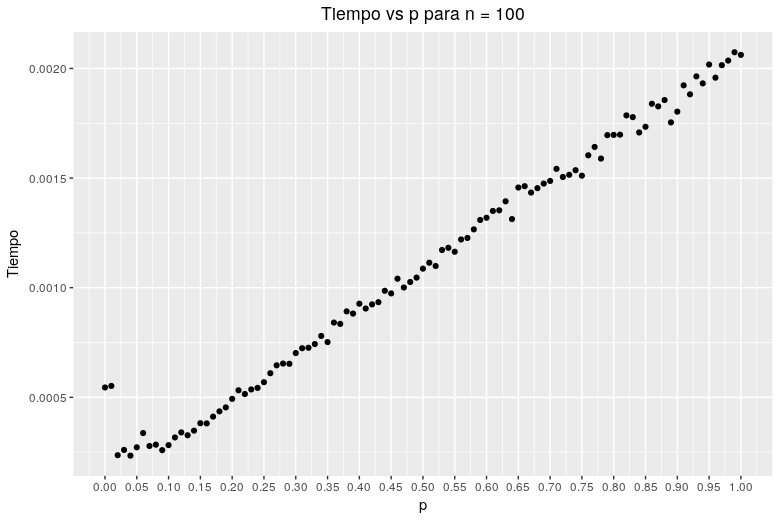
\includegraphics[scale=.80]{plots/plot1n100.png} 
\end{center}
\newpage
\subsection{n = 500}
\begin{center}
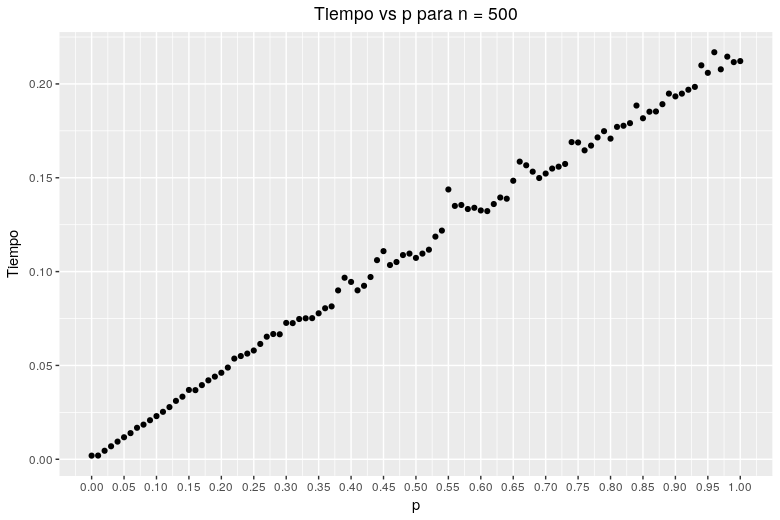
\includegraphics[scale=.80]{plots/plot2n500.png} 
\end{center}
\newpage
\subsection{n = 1000}
\begin{center}
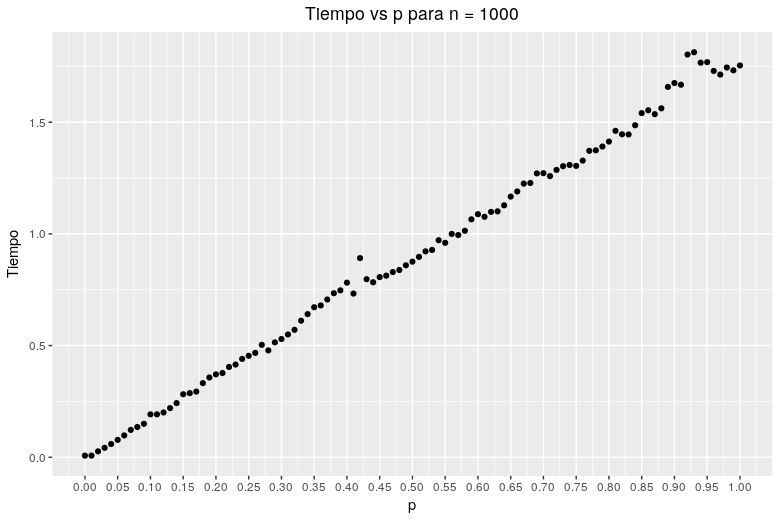
\includegraphics[scale=.80]{plots/plot3n1000.png} 
\end{center}
\newpage
\subsection{n = 10000}
\begin{center}
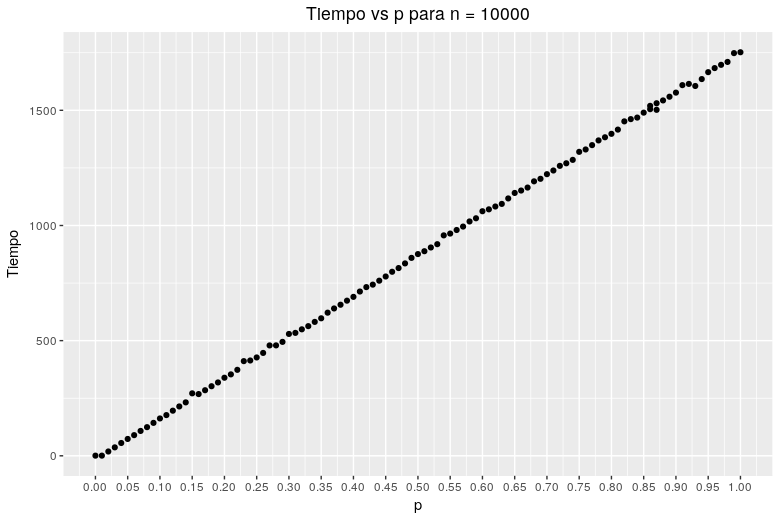
\includegraphics[scale=.80]{plots/plot4n10000.png} 
\end{center}
\newpage
\section{Conclusiones}

Se puede apreciar que ha mayor valor p mayor coste computacional tendrá el algoritmo, pero en contraste los tres primeros gráficos con n = 100, 500 y 1000 se mantuvieron similares en el tiempo, aun así con el último gráfico el tiempo crecio, por lo que a mayor valor de n también es mayor el tiempo de ejecución.

Por lo tanto se puede concluir que a mayor cantidad de vértices y aristas tenga un grafo, mayor será la cantidad de tiempo que se demorara el algoritmo en encontrar un ciclo minimo y un ciclo hamiltoniano.

\end{document}
